\section{Hierarchical clustering}

With K-means clustering we had to predefine the number of clusters $K$. This can be a disadvantage, since we would have to do some initial analysis of the data prior to clustering it. Hierarchical clustering does not require this predefinition. It uses a bottom-up tree algorithm or agglomerative approach to build a dendrogram starting from the observation leaves and ends up combining this into clusters at the trunk. This gives us a flexibility in the number of clusters.

\subsection{Theory}

Agglomerative states that each observation starts in its own cluster and with each iteration of the process are paired with other clusters as we move up the hierarchy.  This is based on a \textit{metric} criteria, a measure of distance between the pairs, and a \textit{linkage} criteria that indicate the dissimilarity between pairwise sets.

A common metric is the Euclidean distance:
\begin{align}
	d(a,b) = \sqrt{\sum_{in=1}^{n} (a_{i} - b_{i})^{2}}  %TODO Christian did you done goof in equation 7.4? with the underlined 2
\end{align}

Which is the straight-line distance between two points in Euclidean space (\textit{n}-space with \textit{n}-tuples of real numbers). Between two points \textit{a} and \textit{b} given by ($X_a$, $Y_a$) and ($X_b$, $Y_b$) the Euclidean distance d(a,b) is:
\begin{align}
	d(a,b) = \sqrt{(X_a - X_b)^2 + (Y_a - Y_b)^2}
\end{align}

Linkage determines which distances to use between sets of observations, i.e. how they are grouped together. \textit{Single} minimizes the distance between the closest elements in clusters, \textit{complete} maximizes distance between the farthest elements, \textit{average} finds the mean of all pairwise distances, and \textit{ward} joins clusters based on the total distance between their centroids. Figure \ref{fig:linkagecriteria} shows the three kinds of linkages to calculate distance.

\begin{figure}[H]
	\centering
	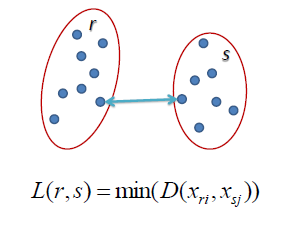
\includegraphics[width=0.3\textwidth]{clusteringMethods/hierarchicalclustering/fig/ClusteringSingle.png}
	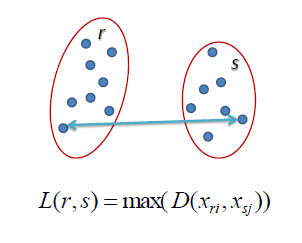
\includegraphics[width=0.3\textwidth]{clusteringMethods/hierarchicalclustering/fig/ClusteringComplete.png}
	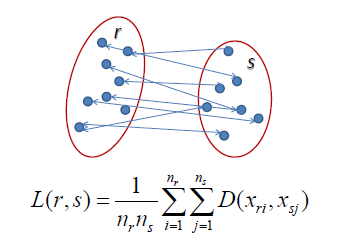
\includegraphics[width=0.3\textwidth]{clusteringMethods/hierarchicalclustering/fig/ClusteringAverage.png}
	\caption{The single, complete and average linkage criteria.}
	\label{fig:linkagecriteria}
\end{figure}

The algorithmic steps for hierarchical clustering are:

1. Start with \textit{N} clusters, one for each data point. \\
2. Merge the clusters that are closest to each other. This gives \textit{N-1} clusters. \\
3. Calculate the distance between the clusters using a linkage criteria (complete, single etc.) \\
4. Repeat step 2 and 3 until we end up with one cluster with \textit{N} data points. The end result is a dendrogram picturing the distance (clusters) as a function of the observations (labels).

\subsection{Results}
\subsubsection*{LAB 10.5.2}
Lab 10.5.2\footnote{Appendix 16 - 10.5.2 Hierarchical Clustering} is using hierarchical clustering to group a 50 x 50 matrix of random observations using Euclidean distance and complete linkage in to two clusters. The AgglomerativeClustering package from Sklearn provides agglomerative clustering functionality in Python to recursively merge pairs of clusters.The Agglomerative Clustering gives the following output.

\noindent\textit{Labels:[1 0 1 1 0 0 0 0 0 0 1 0 0 0 1 0 0 1 10]}

\noindent\textit{No. leaves:  20}

\noindent\textit{No. clusters:  2}


\noindent labels from the complete agglomerative clustering process show how the observations are grouped, starting from $X_i$ to $X_n$. A label [0 1 1 1 0] says observation $X_0$ belongs to the first final cluster, $X_1$ to the second final cluster, $X_2$ to the second etc. The number of leaves correspond to the observations points ($X_a$, $Y_a$). We then generate a dendrogram to picture the Euclidean distance between clusters and their labels. Figure \ref{fig:dendrogramcluster} shows the dendrograms of the three performed clusterings.

\begin{figure}[H]
	\centering
	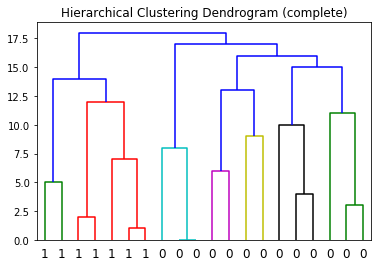
\includegraphics[width=0.3\textwidth]{clusteringMethods/hierarchicalclustering/fig/CompleteClustering.png}
	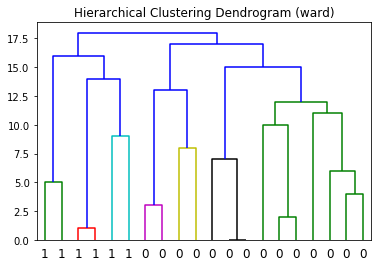
\includegraphics[width=0.3\textwidth]{clusteringMethods/hierarchicalclustering/fig/WardClustering.png}
	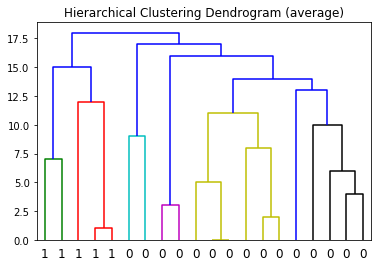
\includegraphics[width=0.3\textwidth]{clusteringMethods/hierarchicalclustering/fig/AverageClustering.png}
	\caption{Dendrograms for complete, ward and average clustering.}
	\label{fig:dendrogramcluster}
\end{figure}

\noindent Also in Figure \ref{fig:dendrogramcluster} is sowing that hierarchical clustering correctly identifies the lower left cluster and the lower right one, however with ward and average a significant euclidean distance has to be reached for it to split correctly, whereas complete splits the observations into two separate ones early on. 

%TODO What is a ward Christian?








